\documentclass[letterpaper,12pt,oneside]{book}
\usepackage[top=1in, left=0.9in, right=0.9in, bottom=1in]{geometry}
\usepackage[utf8]{inputenc}
\usepackage[T1]{fontenc}
\usepackage[spanish,es-nodecimaldot,es-tabla]{babel}
\usepackage{graphicx}
\usepackage{tikz} 
\usepackage{tocloft}
\graphicspath{{./figs/}}
\usepackage{setspace}
\usepackage{fancyhdr}
\usepackage{subcaption}



\begin{document}

    \begin{titlepage}
        \thispagestyle{empty}
        \begin{minipage}[c][0.17\textheight][c]{0.25\textwidth}
            \begin{center}
                
\includegraphics[width=3.5cm, height=3.5cm]{Escudo-UNAM.pdf}
            \end{center}
        \end{minipage}
        \begin{minipage}[c][0.195\textheight][t]{0.75\textwidth}
            \begin{center}
                \vspace{0.3cm}
                \textbf{\textsc{\large Universidad Nacional Aut\'onoma de M\'exico}}\\[0.5cm]
                \vspace{0.3cm}
                \hrule height2.5pt
                \vspace{.2cm}
                \hrule height1pt
                \vspace{1.2cm}
                \textbf{\textsc{\large Facultad de Ciencias}}\\[0.5cm] %
            \end{center}
        \end{minipage}

        \begin{minipage}[c][0.81\textheight][t]{0.25\textwidth}
            \vspace*{5mm}
            \begin{center}
                \hskip2.0mm
                \vrule width1pt height13cm 
                \vspace{5mm}
                \hskip2pt
                \vrule width2.5pt height13cm
                \hskip2mm
                \vrule width1pt height13cm \\
                \vspace{5mm}
                
\includegraphics[height=4.0cm]{Escudo-FCIENCIAS.pdf}
            \end{center}
        \end{minipage}
        \begin{minipage}[c][0.81\textheight][t]{0.75\textwidth}
            \begin{center}
                \vspace{0.5cm}

                {\large\scshape Apoyo a la Investigación (Adquisición y caracterización de imágenes
                mediante un sistema de Ultrasonido clínico)}

                \vspace{2cm}            

                \textsc{\large Manual de usuario }\\[1.5cm]

                \textbf{\textsc{\Large Servicio Social}}\\[2 cm]
                \textsc{\Large p r e s e n t a :}\\[0.5cm]
                \textbf{\textsc{\large {Diego Medel Garduño}}}\\[2cm]          

                \vspace{0.5cm}

                {\large\scshape Tutor:\\[0.3cm] {Dr. Rodrigo Alfonso Martín Salas}}\\[.2in]

                \vspace{0.5cm}

                \large{Ciudad Universitaria, CDMX,}{ }{2024}
            \end{center}
        \end{minipage}
    \end{titlepage}




\tableofcontents
\mainmatter

\chapter{Ultrasonido clinico EDAN modelo DUS 60}

\section{Descripción general del equipo}


\begin{figure}[h!]
    \centering
    \begin{minipage}[b]{0.45\textwidth}
        \centering
        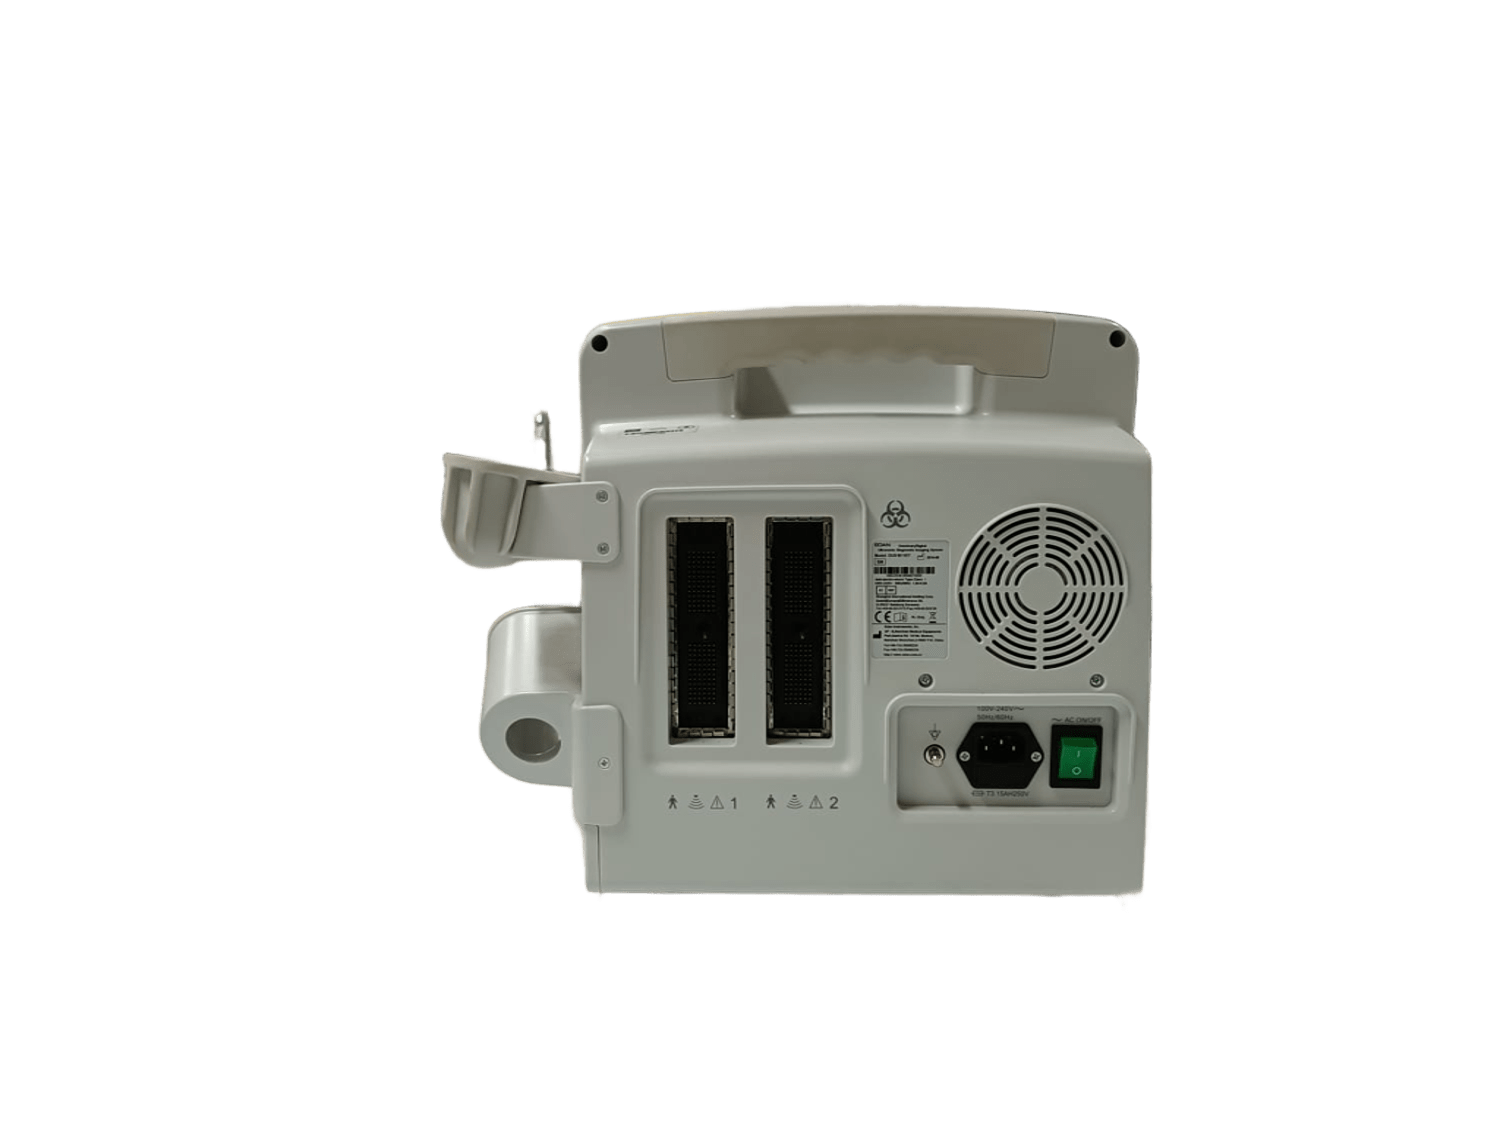
\includegraphics[width=\textwidth]{im24.png}
        \caption{Vista posterior}
        \label{fig:imagen1}
    \end{minipage}
    \hfill
    \begin{minipage}[b]{0.45\textwidth}
        \centering
        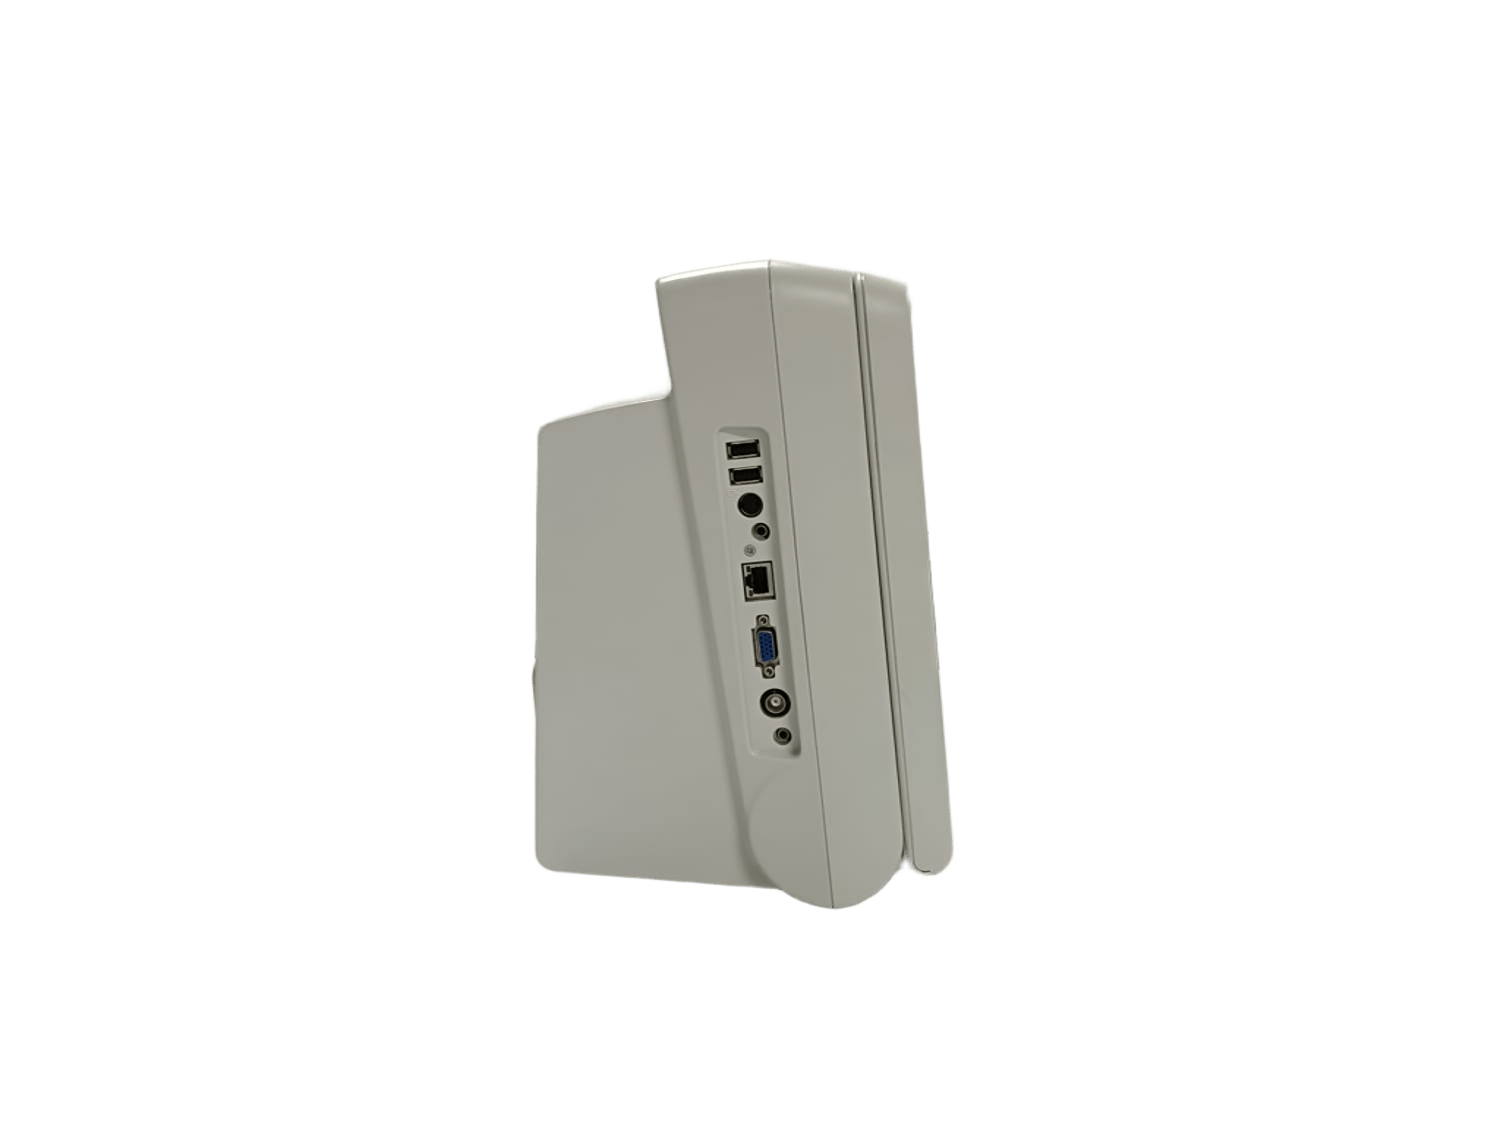
\includegraphics[width=\textwidth]{im25.png}
        \caption{Vista lateral}
        \label{fig:imagen2}
    \end{minipage}
    
    \vspace{0.5cm}
    
    \begin{minipage}[b]{0.45\textwidth}
        \centering
        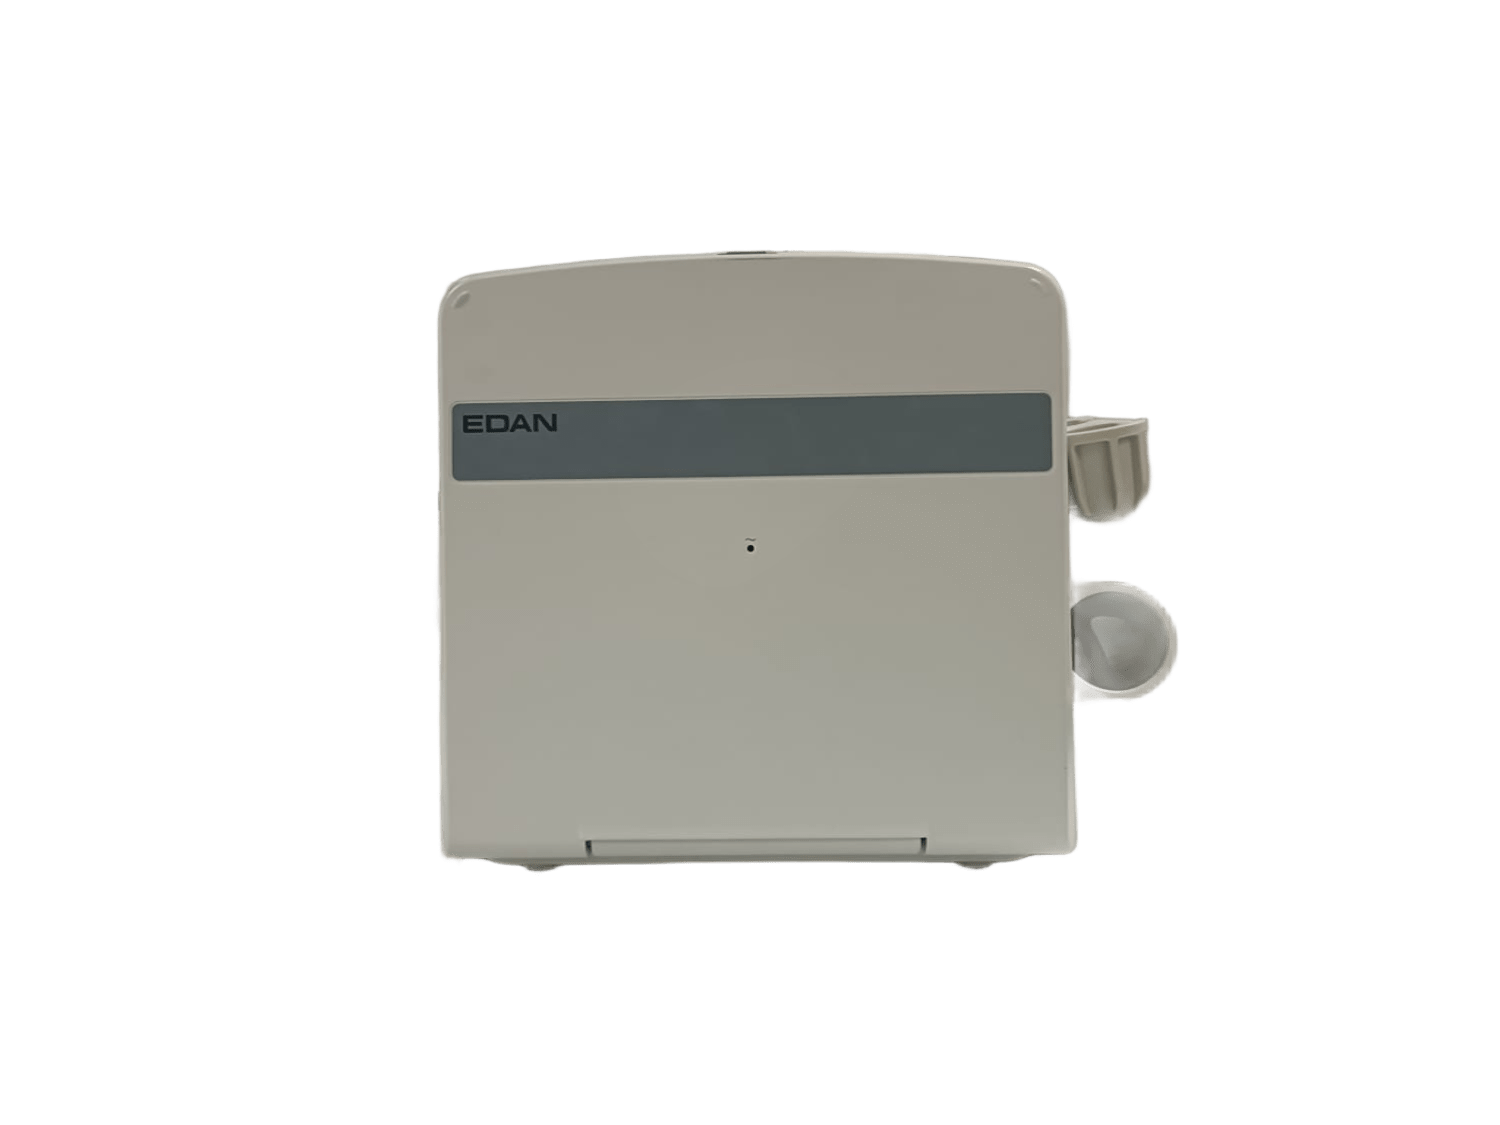
\includegraphics[width=\textwidth]{im23.png}
        \caption{Vista anterior}
        \label{fig:imagen3}
    \end{minipage}
    \hfill
    \begin{minipage}[b]{0.45\textwidth}
        \centering
        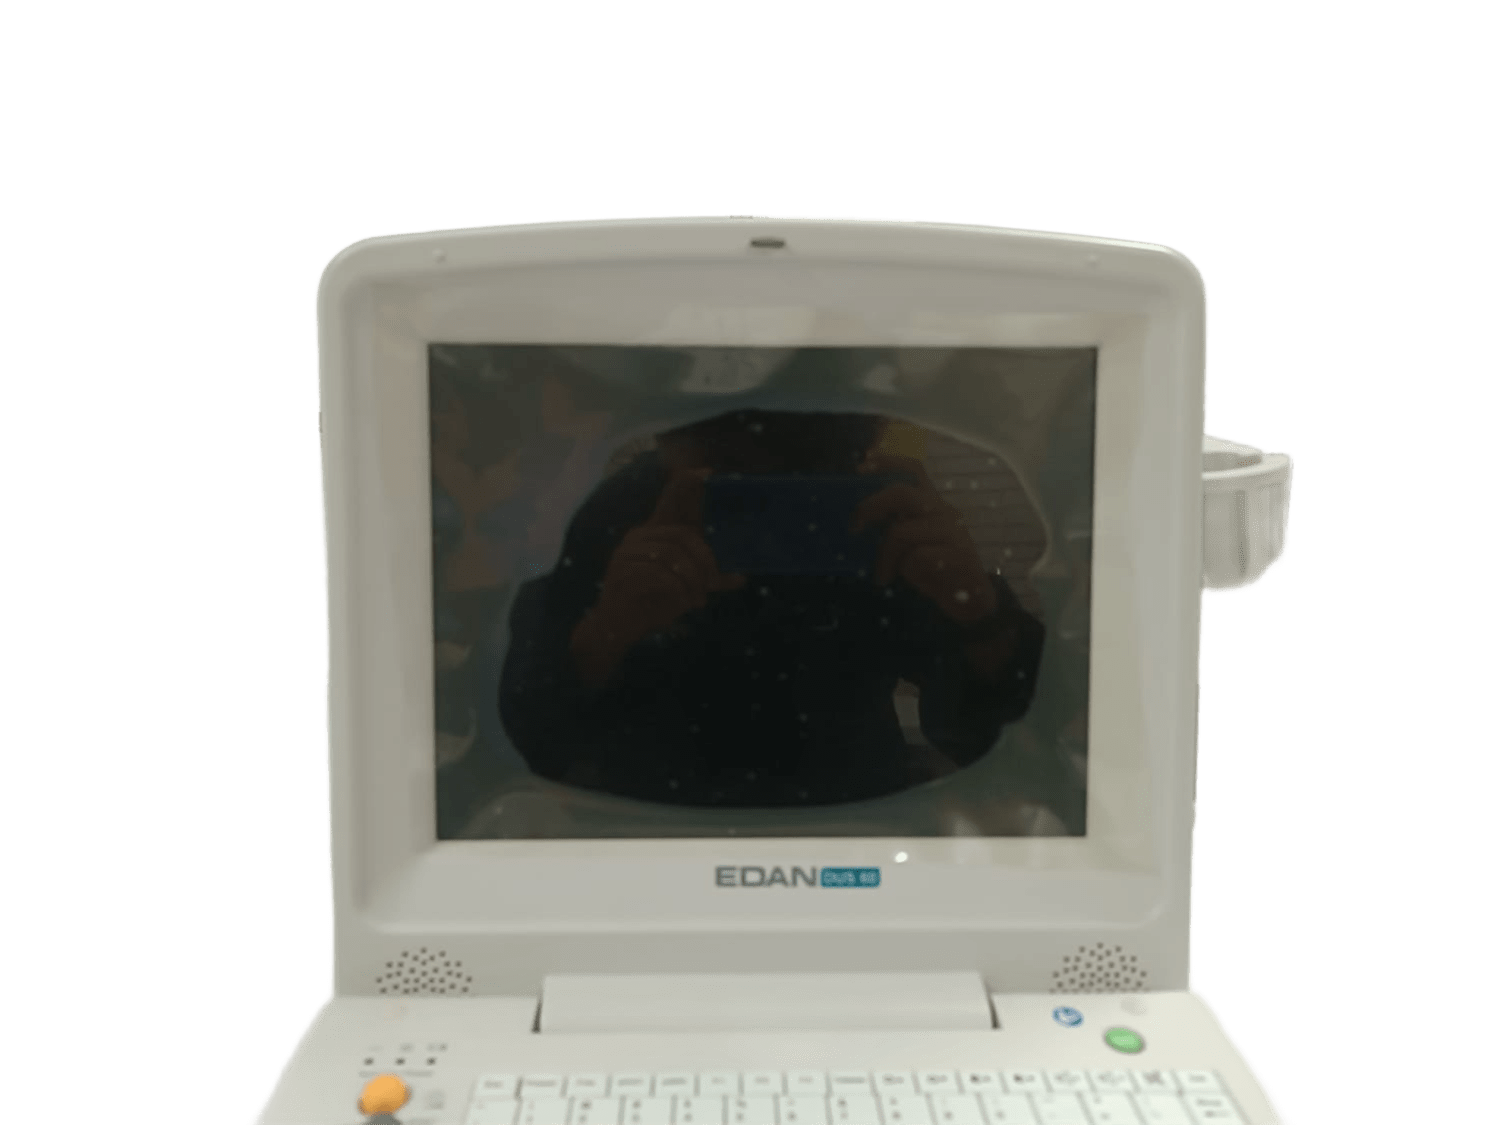
\includegraphics[width=\textwidth]{im21.png}
        \caption{Vista interior}
        \label{fig:imagen4}
    \end{minipage}

    \caption{Vista posterior, lateral, anterior e interior del equipo de ultrasonido clínico de uso veterinario EDAN modelo DUS 60.}
    \label{fig:cuatro_imagenes}
\end{figure}


El sistema de ultrasonido con fines de diagnostico por imagen en pacientes veterinarios EDAN modelo DUS 60 esta diseñado con el fin de obtener imagenes no invasivas de pacientes animales, es compacto y de uso portatil, cuenta con distintos transductores diseñados con el fin de ofrecer distintas maneras de observas el interior de los pacientes. En la figura \ref{fig:cuatro_imagenes} se presentan las tres vistas exteriores del sistema de diagnostico y una vista interior del dispositivo para conocer de manera espacial la distribución de sus aditamentos. 

\vspace{10pt}


En la vista posterior considerada una con las que se debe tener la mayor atención al manejo, cuenta con dos puertos, repletos de pines, que es donde se conectan los transductores, estos dos puertos deben ser tratados de manera cuidadosa ya que el mal uso pueden suponer que el sistema fuera de inutilizable. En esta misma vista se encuentra el puerto para conectar el cable de poder, el boton de encendido y la salida del ventilador. De igual forma es posible observar desde esta vista que el sistema de ultrasonido cuenta con distintos elementos que permiten la colocación de los transductores de manera comoda para quien maneje el equipo.

\vspace{10pt}

En la vista lateral izquierda es posible observar una serie de puertos destinados a la visualización de las imagenes de manera externa o el almacenamiento de las imagenes obtenidas. Los puertos que posee permiten desde colocar un extensión de impresión de imagenes, hasta la visualización en elementos externos como monitores o televisiones. Algo a destacar de esta vista es la presencia de puertos USB los cuales tienen la función de introducir o extraer imagenes en distintos formatos como jpg, png, bmp, entre otros. 

\vspace{10pt}


Por otro lado se encuentra la vista anterior, que no cuentan con elementos distinguibles con alguna función especifica, sino que solo considera la carcasa protectora de la pantalla del dispositivo, esta misma carcasa funge como panel de control, ya que en ella se encuentra el sistema que permite la navegación en el dispositivo. En el interior de esta carcasa se encuentran los elementos que se pueden observar en la figura \ref{fig:imagen4}, que componen la vista interior del sistema de ultrasonido. De manera general se observa que la vista interior esta compuesta por una pantalla y un teclado, de manera más particular esta pantalla es la encargada de desplegar las imágenes de ultrasonido en distintos modos que sean obtenidas posteriormente. Por su parte el denominado teclado constituye el panel de control, puesto que no solo esta conformado por teclas con elementos alfanumerios, sino en el panel de control tambien existen elementos para modificar la imagen, como la ganancia, modificar el constraste en ciertas zonas de la imagen, realizar acercamientos, modificar el modo de estudio y otras más. Es importante destacar que este sistema no cuenta con ningun tipo de elemento externo para la navegación, en cambio el panel de control cuenta con su propio elemento de navegación, que no es tactil, se trata de una esfera. 

\section{Carácteristicas especificas del equipo}

\subsection{Encendido}

El encendido del equipo consta de tres procesos principales, entre ellos se encuentra en conectar el cable de poder desde su terminal, hasta la toma de corriente, para esto en la figura \ref{fig:imagen1} donde se observa la vista posterior, se observa en la parte inferior derecha una sección con un apagador de color verde, a su lado izquierdo se encuentra la terminal de cable de poder. Una vez conectada a la corriente, es importante que el apagador de color verde a la derecha del cable de poder se mantenga apagado, esto se puede identificar ya que cuando esta prendido emite una luz, otro referente es que el apagador esta posicionado hacia abajo.

\vspace{10pt}



\begin{figure}[h!]
    \centering
    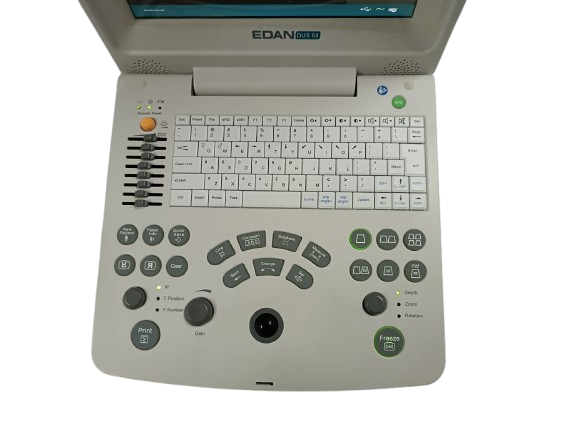
\includegraphics[scale = 0.45]{im17.png}
    \caption{Panel de control}
    \label{fig:panel}
    
\end{figure}


\vspace{10pt}

El manual oficial del equipo especifica que antes de dejar que la corriente fluya a traves del equipo se deben conectar los distintos transductores que se van a utilizar, esto para evitar que cualquier daño en los piezoelectricos. Una vez que se hayan conectado los transductores, el switch de color verde debe encenderse, como se menciono, prueba de que esta dejando pasar corriente es que emite luz, en la figura \ref{fig:panel} se presenta el panel de control de manera completa, en la esquina superior derecha se haya un boton de color verde, que al presionarlo permite que el dispositivo encienda. Una forma de verificar de que el sistema esta encendido es que el ventilador comienza sus operaciones emitiendo de manera sonora un sonido, otra señal es que en la pantalla se despliega un logo con que indica que el producto es de la marca EDAN.


\subsection{Elementos de la pantalla}

Una vez encendido el dispositivo habrá un despliegue de inicio en la pantalla como el que se puede observar en la figura \ref{fig:pantalla}. Esta pantalla cuenta con distintas secciones, esto de igual manera se aprecia mejor en el grafico anteriomente referido. En la parte superior izquierda se despliegan los datos respeto al paciente, como su nombre y su número asociado que lo identifica, en esa misma región, pero del lado derecho se encuentran los elementos propios del transductor como la ganancia, la frecuencia que utiliza y el modelo, es importante mencionar que cada uno de los transductores que se pueden utilizar tienen asociado un rango de frecuencias que de las que se pueden hacer uso, este rango es particular para el tipo y modelo de transductor. 


\begin{figure}[h!]
    \centering
    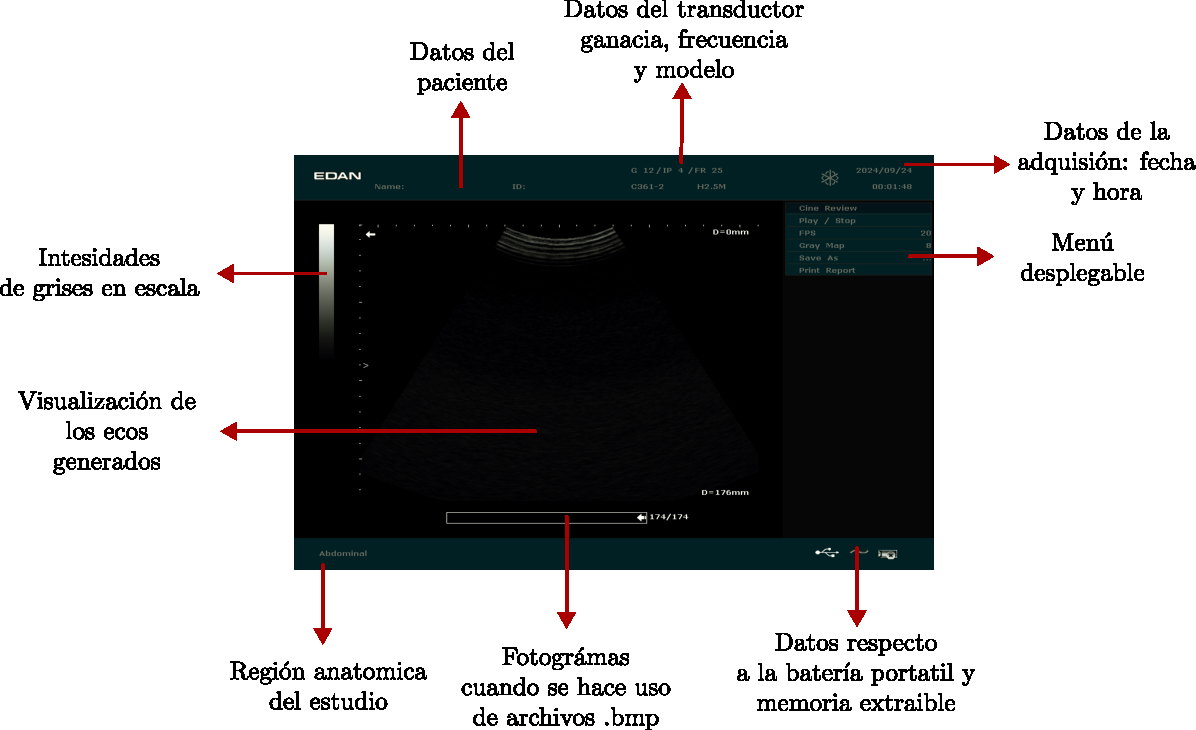
\includegraphics[scale = 0.75]{im13.pdf}
    \caption{Pantalla}
    \label{fig:pantalla}
\end{figure}



\vspace{10pt}

En la esquina superior derecha se encuentran los elementos que distinguen la hora y fecha en la que se ha hecho es estudio, la figura \ref{fig:pantalla} es la forma en la que el dispositivo de ultrasonido se encarga de compartir los estudios que ha realizado. Por debajo de la esquina superior derecha se encuentra un menú desplegable, de manera concreta el que se presenta en la figura \ref{fig:pantalla} es el menú correspondiente al modo cine, sin embargo no es el unico menú que existe, ya que cada función o modo del dispositivo tiene asociado un menú desplegable, que muestra cada una de opciones de lo que se puede realizar con cierta función o modo disponible. Por ejemplo en el panel de control existe un boton con la etiqueta \textit{file}, una vez que se oprime este boton se despliegan opciones respectivas al tratamiento de los documentos, como su exportación, importación o almacenamiento. 

\vspace{10pt}


En la esquina inferior derecha se encuentran elementos que señalizan si esta conectada la bateria portatil o si existe un elemento de almacenamiento externo colocado. En la figura \ref{fig:pantalla} se observan en principio dos figuras, una de ellas tiene forma de bateria y como elemento representativo tiene un circulo con una equis en su interior, este dibujo indica que no hay un elemento de bateria portatil, por lo que en caso de no estar conectada a la corriente directa, no hay forma de usarlo. El otro elemento denota el simbolo universal de las memorias USB, por lo que si existe un elemento de almacenamiento externo este elemento aparece, en caso de no tener ningún elemento de almacenamiento externo este elemento no se observa.

\vspace{10pt}


En la parte inferior media se ecuentra una barra que designa el número total de imagenes que se han tomado en un estudio, este elemento esta relacionado con archivos .bmp, considerando el número de imágenes que se han tomado, se puede elegir una la que al criterio de quien este tomando el estudio sea la más adecuada. En la esquina inferior izquierda se encuentra una leyenda que indica la región anatomica en la que se esta haciendo el estudio, este elemento tiene una función descriptiva, ya que si alguien ajeno a la persona que hizo el estudio en un principio recibe una imagen por tecnica de ultrasonido, tenga noción de lo que región es la que esta observando. 

\subsection{Elementos del panel de control}
\subsection{Transductores}





\chapter{Adquisición de imágenes}
\chapter{Analisis estadistico}
\chapter{Presentación y discusión de resultados}
\chapter{Conclusiones}


 
    


\end{document}